\documentclass[]{article}
\usepackage[utf8]{inputenc}


\title{Resumen química I c2}
\author{}
\date{}
\usepackage[spanish]{babel}
\usepackage{amsmath,amsfonts,amssymb,amsthm}
\usepackage{natbib}
\usepackage{graphicx,float}
\usepackage[margin=1.0in]{geometry}
\usepackage{color}


%\newcommand{comando kliao}{comando bueno}
%\DeclareMathOperator\cis{cis}
%\DeclareMathOperator\Arg{Arg}



\begin{document}
\maketitle
\tableofcontents
\clearpage



\part{Clase 11}



\section{Teoría cinética para líquidos y sólidos}
La \textbf{teoría cinética molecular} también puede usarse para explicar de manera cualitativa el comportamiento de las sustancias en \textbf{estado líquido} y en \textbf{estado sólido}.



\subsection{En Gases:}  

\begin{itemize}
	\item La energía cinética promedio de un conjunto de moléculas de gas disminuye conforme baja la temperatura.
	\item Las interacciones entre las moléculas de una gas son despreciables debido a las grandes distancias que separan a las moléculas a presiones y temperaturas ordinarias.
\end{itemize}



\subsection{En líquidos:}  

\begin{itemize}
	\item Las moléculas están tan juntas que hay muy poco espacio vacío, por ello los líquidos son más difíciles de comprimir.
	\item Las fuerzas de atracción entre las partículas son lo suficientemente grandes para que ocurran agrupamientos desordenados.
	\item La energía de movimiento de las partículas de los líquidos es suficiente como para superar en forma parcial las fuerzas de atracción entre ellas.
\end{itemize}



\subsection{En sólidos:}  

\begin{itemize}
	\item Las fuerzas intermoleculares son lo suficientemente fuertes para mantener juntas a las partículas y fijarlas en una posición rígida.
	\item Los sólidos, al igual que los líquidos, no son muy compresibles por que las partículas tienen poco espacio libre entre ellas.
\end{itemize}

Dos factores que influyen en el estado físico de un objeto son la \textbf{temperatura} y la \textbf{presión}.

Primero notemos la diferencia entre:

\begin{itemize}
	\item \textbf{Fuerzas intramoleculares:} mantienen juntos los átomos de una molécula.
	\item \textbf{Fuerzas intermoleculares:} son fuerzas de atracción entre las moléculas (suelen ser más débiles que las anteriores).
\end{itemize}

\begin{figure}[H]
\center
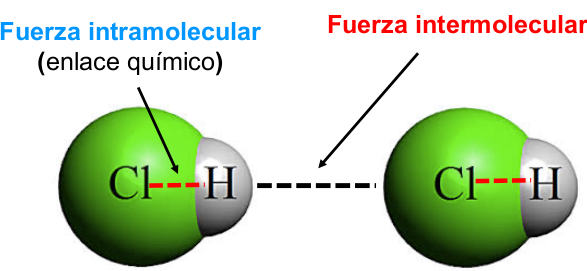
\includegraphics[scale=0.3]{foto/foto4.png}
\caption{Comparación entre fuerzas intramoleculares e intermoleculares.}
\end{figure}

Los puntos de ebullición y fusión reflejan la magnitud de las fuerzas intermoleculares.



\section{Tipos de fuerzas intermoleculares}

\begin{figure}[H]
\center
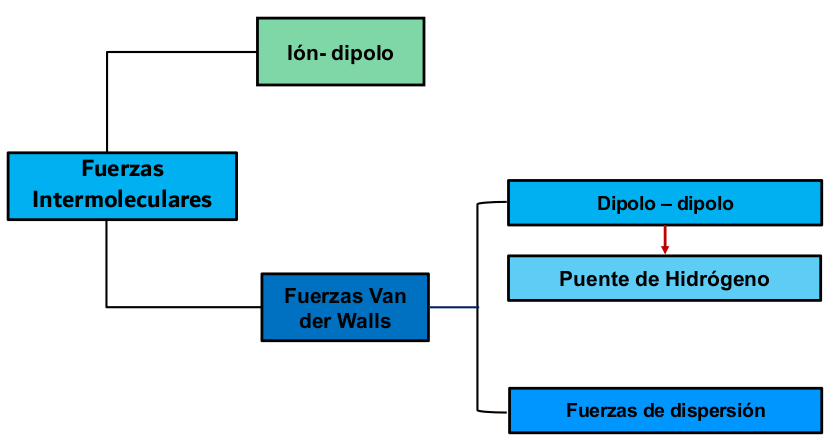
\includegraphics[scale=0.32]{foto/foto5.png}
\caption{Clasificación de las fuerzas intermoleculares.}
\end{figure}



\subsection{Fuerzas ión-dipolo}
Son las fuerzas que atraen entre sí a un ión y la carga parcial de un ezxtremo de una molécula polar

\begin{figure}[H]
\center
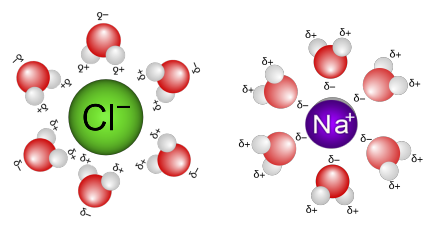
\includegraphics[scale=0.3]{foto/foto6.png}
\caption{Interacción ión-dipolo.}
\end{figure}
 
Magnitud de atracción depende de: carga y tamaño del ión, magnitud del momento dipolar y tamaño de la molécula.



\subsection{Fuerzas dipolo-dipolo}
Fuerza de atracción entre moléculas polares (que poseen momento dipolar). Tienden a alinearse de tal manera que la atracción sea máxima. \textbf{Más débiles que las fuerzas ión-dipolo}.

\begin{figure}[H]
\center
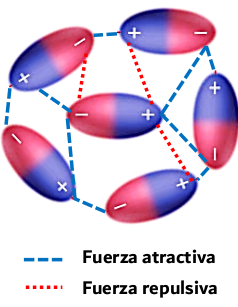
\includegraphics[scale=0.31]{foto/foto7.png}
\caption{Interacción dipolo-dipolo.}
\end{figure}
 
\subsection{Fuerzas de disperción}
Las \textbf{fuerzas de disperción de London} se generan a partir de \textbf{dipolos temporales} inducidos por la fuerza que ejercen otros dipolos o iones. \textbf{Aumentan con la masa molar} (ya que con mayor masa molar se suelen tener más electrones). \textbf{Único tipo de fuerza entre meléculas no polares}.



\subsection{Enlace de hidrógeno}
Tipo especial de interacción \textbf{dipolo-dipolo} entre un átomo de hidrógeno conectado a un átomo muy electronegativo (F, N, O).

\begin{figure}[H]
\center
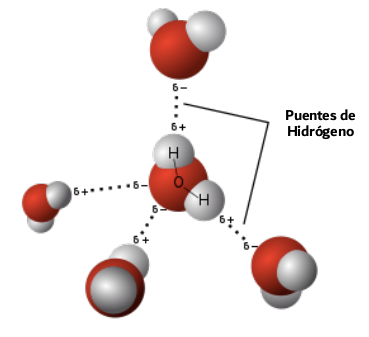
\includegraphics[scale=0.33]{foto/foto8.png}
\caption{Moléculad de agua}
\end{figure}



\subsection{Comparación de fuerzas intermoleculares} 
En general

\begin{center}
ion-dipolo $>$ enlace H $>$ dipolo-dipolo $>$ fuerzas de disperción 
\end{center}

Todas estas interacciones son \textbf{considerablemente más débiles} que los enlaces covalentes y iónicos, los cuales tienen energías en el rango de cientos de kilojoules por
mol.

\begin{figure}[H]
\center
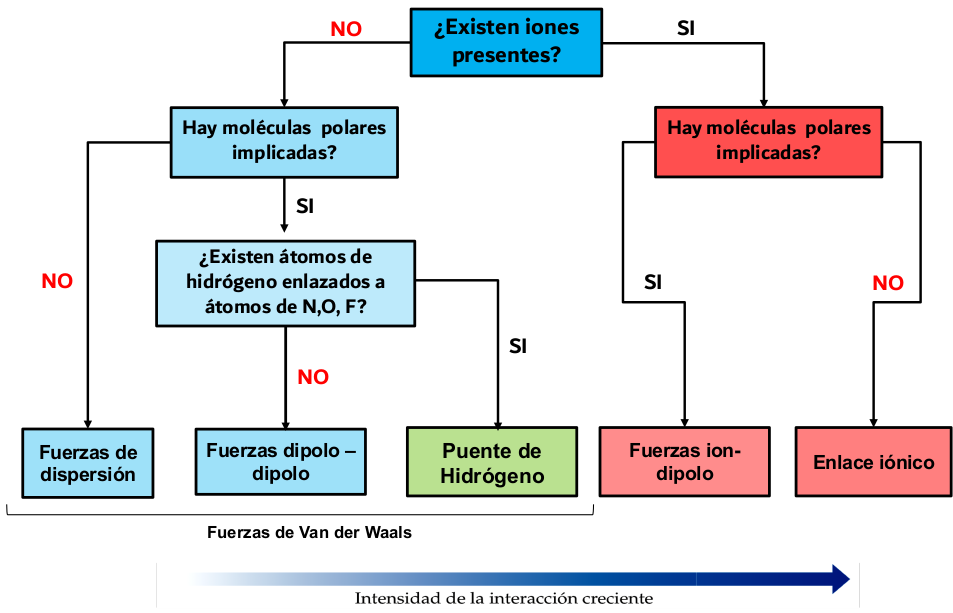
\includegraphics[scale=0.36]{foto/foto9.png}
\caption{lifehack para el certamen.}
\end{figure}



\part{CLase 12}



\section{El estado líquido}
Es un estado en que la materia se presenta como fluído con volumen definido, pero sin forma determinada. No tienen una distribución ordenada.



\section{Propiedades de los líquidos}



\subsubsection{Tensión superficial}
Cantidad de energía necesaria apra estirar o aumentar la superficie de un líquido por unidad de área. La tensión superficial es una medida de la \textbf{fuerza elástica que existe en la superficie de un líquido}. En general, los líquidos que tienen fuerzas intermoleculares grandes también poseen tensiones superficiales altas.

\begin{figure}[H]
\center
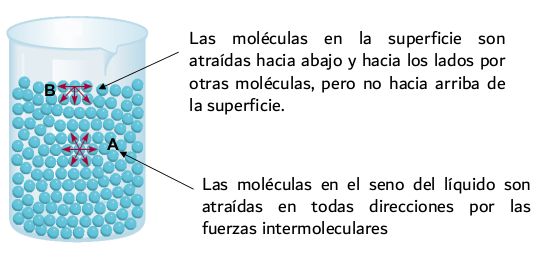
\includegraphics[scale=0.45]{foto/foto10.png}
\end{figure}

La \textbf{acción capilar} es el ascenso de líquidos por una superficie vertical; \textbf{consecuencia de la tensión supeficial}.

\begin{figure}[H]
\center
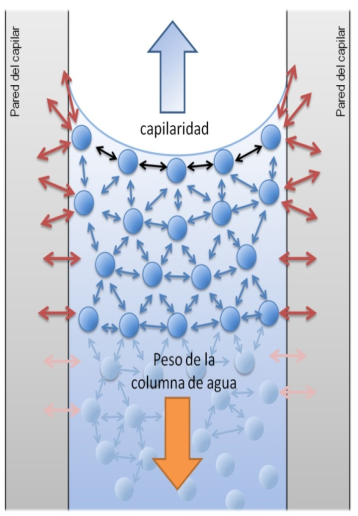
\includegraphics[scale=0.3]{foto/foto11.png}
\caption{acción capilar}
\end{figure}

En el capilar el agua sube hasta que las fuerzas de cohesion (flechas azul y negro), adhesion (flecha roja) y peso se equilibran. El agua sube por los tallos de las plantas usando la acción capilar (capilares). 

\begin{itemize}
	\item \textbf{menisco cóncavo:} Fuerzas de adhesión $>$ cohesión.
	\item \textbf{menisco convexo:} fuerzas de cohesión $>$ adhesión.
\end{itemize}

\begin{figure}[H]
\center
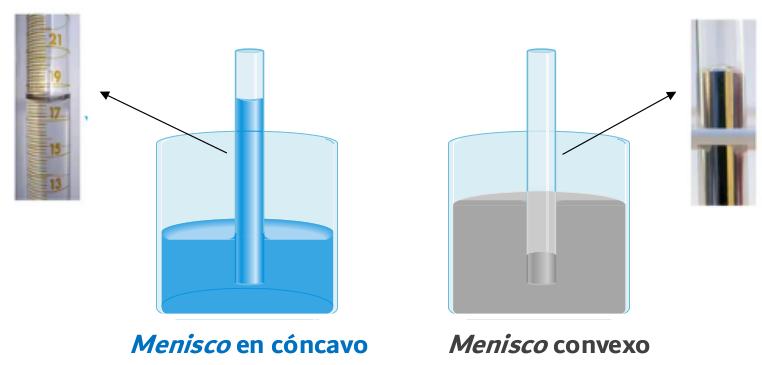
\includegraphics[scale=0.3]{foto/foto12.png}
\caption{Efectos de fuerzas de adhesión y cohesión}
\end{figure}



\subsection{Viscosidad}
Medida de la \textbf{resistencia} de un líquido a fluir; cuando más viscozo, más lento es su flujo. Las \textbf{fuerzas intermoleculares fuertes} provocan líquidos \textbf{más viscosos} que los que tienen fuerzas intermoleculares débiles. Entre compuestos análogos, la viscosidad aumenta al incrementarse la masa molar. La viscosidad \textbf{disminuye al aumentar la temperatura}.



\subsection{Presión de vapor y punto de ebullición}
Es la presión ejercida por las partículas de vapor en equilibrio dinámico con la fase líquida a una temperatura determinada.

\begin{figure}[H]
\center
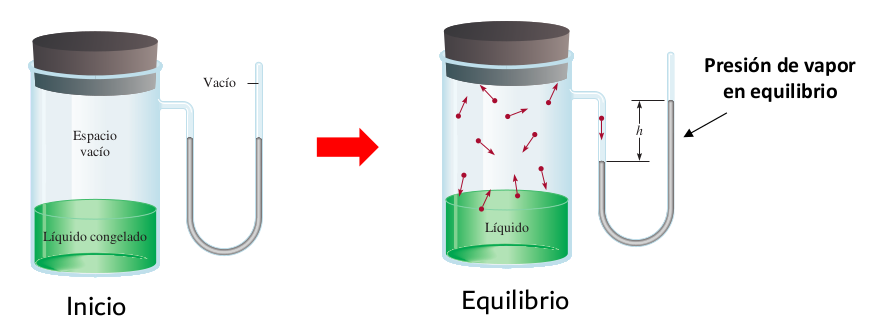
\includegraphics[scale=0.35]{foto/foto13.png}
\caption{Como medir la presión de vapor.}
\end{figure}

Presion de vapor \textbf{depende de las características de la sustancia y de su temperatúra}. A medida que aumenta la temperatura aumentan las particulas que pasan a la fase de vapor, por lo tanto la presión aumenta; si la sustancia se atrae fuertemente entre si (fuerzas intermoleculares), la presion de vapor será más baja.

\begin{figure}[H]
\center
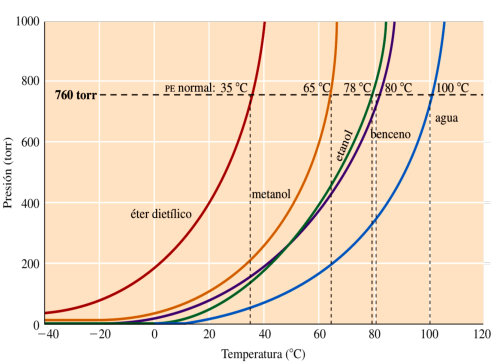
\includegraphics[scale=0.35]{foto/foto14.png}
\caption{presion de vapor vs temperatura}
\end{figure}

El \textbf{punto de ebullición} es la temperatura a la cual la presion de vapor de un líquido iguala a la presión atmosférica externa (a diferentes alturas el agua ebulle a diferente temperatura).

\begin{figure}[H]
\center
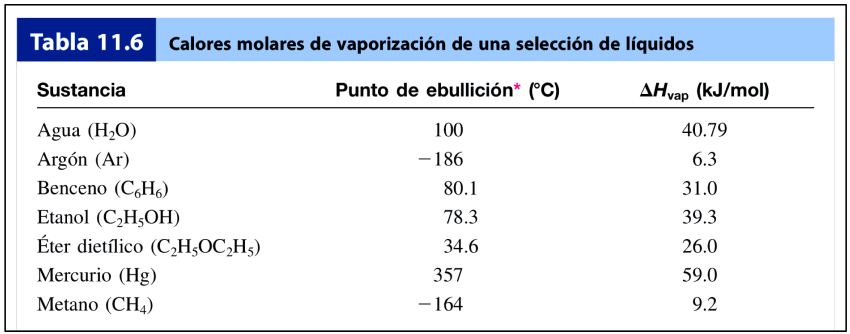
\includegraphics[scale=0.37]{foto/foto15.png}
\caption{temperaturas de ebullición.}
\end{figure}



\section{Propiedades del agua}

\begin{itemize}
	\item Sustancia líquida más abundante en la tierra.
	\item Imprescindible para los procesos bioquímicos.
	\item Disolvente universal (solvente polar).
	\item Elevado calor especifico (mucho calor para cambiar la temperatura). En la naturaleza se ve que los animales la usan para regular la temperatura.
	\item Agua en estado sólido es menos denso que en estado líquido; explicación de por qué el hielo flota (estructura de cristal de hielo es ordenada; tetraedro).
\end{itemize}

\begin{figure}[H]
\center
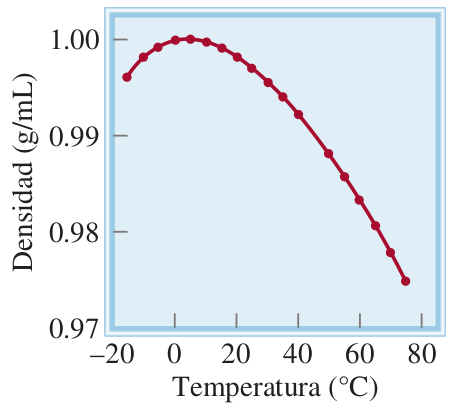
\includegraphics[scale=0.38]{foto/foto16.png}
\caption{Densidad del agua con respecto a la temperatura}
\end{figure}


\part{Clase 13}



\section{El estado sólido}



\subsection{Sólidos cristalinos}
Un \textbf{sólido cristalino} posee un ordenamiento estricto y regular, es decir, sus átomos, moléculas o iones ocupan posiciones específicas. Las fuerzas que mantienen la estabilidad de un cristal pueden ser iónicas, covalentes, de van der waaals, puntes de hidrogeno o una combinación de ellas.

\begin{itemize}
	\item La distribución de las particulas en solidos cristalinos maximisa las fuerzas netas de atracción molecular.
	\item Los sólidos cristalinos suelen tener superficies planas que forman ángulos entre si.
	\item Ejemplos: Cloruro de sodio, cristal de cuarzo, diamante.
\end{itemize}

Una celda unitaria es la unidad básica que se repite en un sólido cristalino; tiene ángulos y aristas. Existen varios tipos de celdas unitarias:

\begin{enumerate}
	\item cúbica (fluorita)
	\item tetragonal (calcopirita)
	\item ortorrómbica (aragonita)
	\item romboédrica (calcita)
	\item hexagonal (esmeralda)
	\item monoclínica (azurita)
	\item triclínica (rodonita)
\end{enumerate}

Hay tres tipos de celdas cúbicas: cúbica simple, cúbica centrada en el cuerpo, cúbica centrada en las caras (la más compacta).



\subsubsection{Cristales iónicos}
Formado por iones (ejemplo Cloruro de sodio). Unidos por atracción \textbf{electroestática}.

\begin{itemize}
	\item Formados for especies cargadas
	\item Aniones y cationes suelen ser de distinto tamaño
	\item Se mantienen unidos por enlaces iónicos
	\item Suelen tener \textbf{puntos de ebullición elevados}
	\item \textbf{No conducen electricidad}. En estado fundido o disueltos en agua conduce electricidad (electrolito)
	\item Son duros (resistentes al rayado) y frágiles (se rompen facilmente)
\end{itemize}



\subsubsection{Cristales covalentes}
Átomos unidos en grandes redes por \textbf{enlaces covalentes} (ejemplo: los dos alótropos del carbono, diamante y grafito).

Estructura cristalina del diamante:

\begin{itemize}
	\item cada átomo está enlazado de manera tetraédrica a otros 4 átomos de carbono
	\item los enlaces covalentes fuertez le otorgan gran resistencia y un elevado punto de fusión
\end{itemize}

Estructura cristalina del grafito:

\begin{itemize}
	\item átomos se distribuyen en forma de anillos hexagonales, cada uno enlazado a otros 3.
	\item se mantienen unidos por fuerzas débiles de van der waals por lo que sep ueden deslizar entre sí.
\end{itemize}

Los cristales covalentes poseen las siguientes caracteristicas.

\begin{itemize}
	\item son duros
	\item malos conductores eléctricos
	\item insolubles en todos los disolventes comuntes
	\item puntos de fusión muy altos
\end{itemize}



\subsubsection{Sólidos moleculares}
Unidos por fuerzas \textbf{dipolo-dipolo}, fuerzas de \textbf{disperción} o \textbf{enlaces de hidrógeno}.

\begin{itemize}
	\item son mas suaves y quebradizos que los cristales iónicos o covalentes
	\item puntos de fusión relativamente bajos (casi siempre $<200^{\circ} C$)
	\item sunstanticas que son gases y líquidos a temperatura ambiente pueden formar sólidos moleculares a temperaturas bajas.
\end{itemize}



\subsubsection{Cristales metálicos}
Formado por metales, su empaquetamiento suele ser muy denso (modelo de mar de electrones; \textbf{deslocalización electrónica}). Son resistentes y buenos conductores de calor y electricidad.
%%%% añadir lo que falta


\subsection{Sólidos amorfos}

\begin{itemize}
	\item estructuras similares a la de los líquidos, pero sus particulas carecen de la libertad de movimiento de estos.
	\item No tienen caras bien definidas.
\end{itemize}



\subsubsection{El vidrio}
El vidrio es un producto de fusión de materiales inorgánicos ópticamente transparente que se ha enfriado a un estado rígido sin cristalizar.
El vidrio es una mezcla fundida de dióxido de silicio (SiO 2 ), su principal componente, y
otros compuestos como óxido de sodio ($Na_2O$), óxido de boro ($B_2O_3$) y ciertos óxidos de
metales de transición que le confieren color y otras propiedades.

\begin{figure}[H]
\center
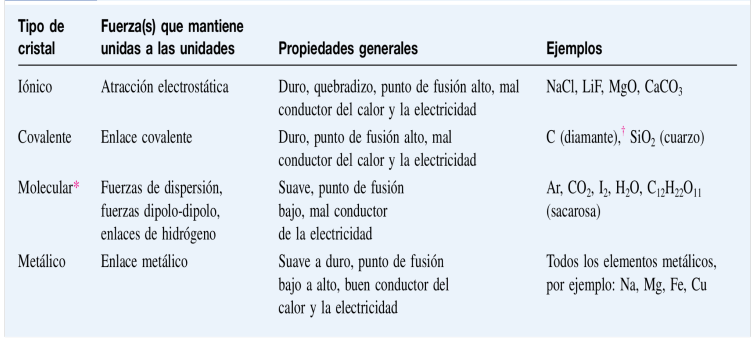
\includegraphics[scale=0.53]{foto/foto3.png}
\caption{Tipos de cristales y propiedades generales}
\end{figure}



\section{Disoluciones}
Es una mezcla homogénea de dos o mas sustancias. Compuesta por soluto (menor cantidad) y solvente (mayor cantidad). Segun la capacidad de disolver soluto se pueden clasificar en:

\begin{itemize}
	\item \textbf{Disolución no saturada:} contiene menor soluto que el que puede disolver.
	\item \textbf{Disolución saturada:} contiene máxima cantidad de soluto que puede disolver.
	\item \textbf{Disolución sobresaturada:} contiene más soluto del que puede disolver.
\end{itemize}



\subsection{Análisis molecular del proceso de disolución}
\begin{enumerate}
	\item Separación particulas de disolvente.
	\item partículas de soluto se disocian en disolvente.
	\item partículas se mezclan formando la disolucion; las estapas 1 y 2 requieren de energía para romper las fuerzas de atracción intermoleculares.
\end{enumerate}
%%%%%%%55 determinar si se deberian agregar als ecuaciones 


\subsection{Factores que afectan la solubilidad}
La \textbf{solubilidad} es la máxima cantidad de soluto que un disolvente puede disolver a una \textbf{temperatura específica}



\subsubsection{Efectos de la temperatura}
En los \textbf{sólidos}, la solubilidad aumenta al incrementarse la temperatura de disolución (con excepciones). 
 
\begin{figure}[H]
\center
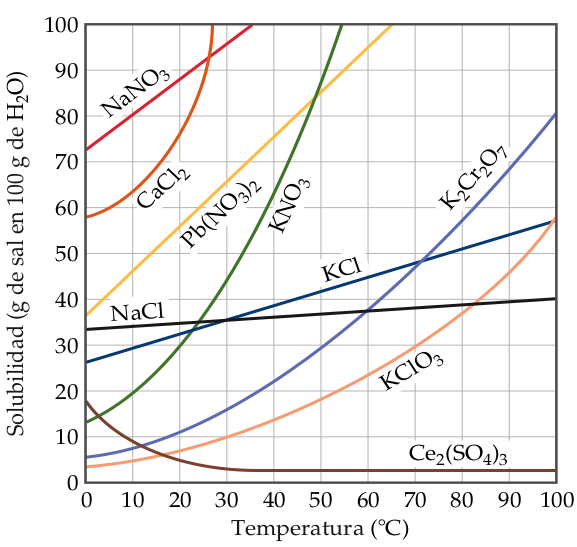
\includegraphics[scale=0.3]{foto/foto1.png}
\caption{efecto de la temperatura en la solubilidad de algunos sólidos en agua.}
\end{figure}

La solubilidad de los \textbf{gases} en agua disminuye con la temperatura.

\begin{figure}[h]
\center
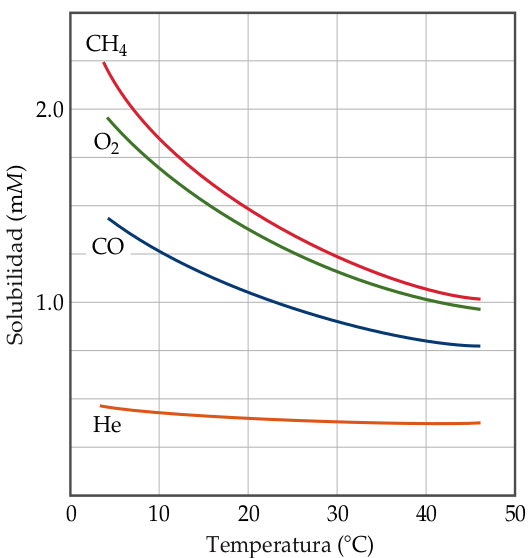
\includegraphics[scale=0.3]{foto/foto2.png}
\caption{efecto de la solubilidad de algunoas gases en agua con la temperatura.}
\end{figure}



\subsubsection{Efectos de la presión}
Las solubilidades de los sólidos y líquidos no muestran un efecto apreciable de presión, mientras que la solubilidad de un gas en cualquier disolvente aumenta al incrementar la presión del gas sobre el disolvente. La \textbf{ley de Henry} establece que la solubilidad de una gas en un líquido es proporcional a la presión del gas sobre la disolución:

\begin{equation}
c \varpropto kP  \Rightarrow c=kP
\end{equation}

donde $c$ es la concentración en $mol/L$, $P$ es la presión en atm y $K$ es una constante que depende de la temperatura del sistema. 



\part{Clase 14}



\section{Propiedades coligativas}
Son propiedades que dependen sólo del \textbf{número de particulas} de un soluto en la disolución y no de la naturaleza de las partículas del soluto (coligativo, que depende del efecto colectivo). Son independientes del tipo de soluto que hayamos introducido en la disolución, solo dependen de su cantidad de particulas.

\begin{itemize}
	\item Disminución de la presión de vapor
	\item Aumento del punto de ebullición
	\item Disminución del punto de congelación
	\item Presión osmótica
\end{itemize}



\subsection{Disminución de la presión de vapor}

\begin{figure}[H]
\center
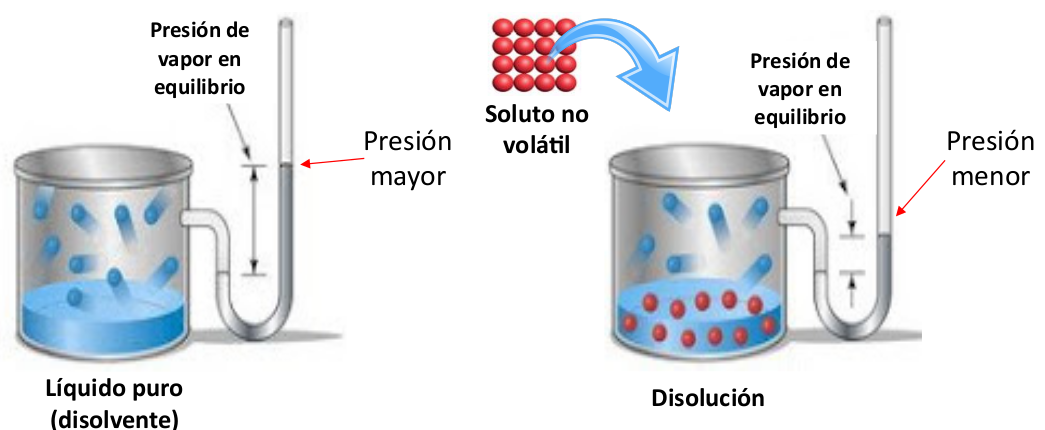
\includegraphics[scale=0.33]{foto/foto17.png}
\caption{La presión de vapor disminuye al agregar soluto}		
\end{figure}

\subsubsection{Ley de Raoult}
Establece que la presión parcial de un disolvente en una disolución ($P_{1}$) está dada por la presión de vapor del disolvente puro ($P_{1}^{\circ}$) multiplicada por la fraccion molar del disolvente en la disolución ($X_{1}$).

\begin{equation}
P_{1}=X_{1}P_{1}^{\circ}
\end{equation}

En donde $X_{1}$: fracción molar del \textbf{disolvente} y $X_{2}$: fracción molar del \textbf{soluto} 

\begin{center}
	$X_{1}+X_{2}=1 \rightarrow X_{1}=1-X_{2}$ \\
	$P_{1}=(1-X_{2})P_{1}^{\circ} \rightarrow P_{1}=P_{1}^{\circ} - X_{2}P_{1}^{\circ}$
\end{center}

con esto obtenemos

\begin{equation}
P_{1}^{\circ}-P_{1}=\Delta P= X_{2}P_{1}^{\circ}
\end{equation}



\subsection{Aumento del punto de ebullición}
Punto de ebullición: temperatura a la cual la presión de vapor de un líquido se iguala a la presión atmosférica externa.

\begin{figure}[H]
\center
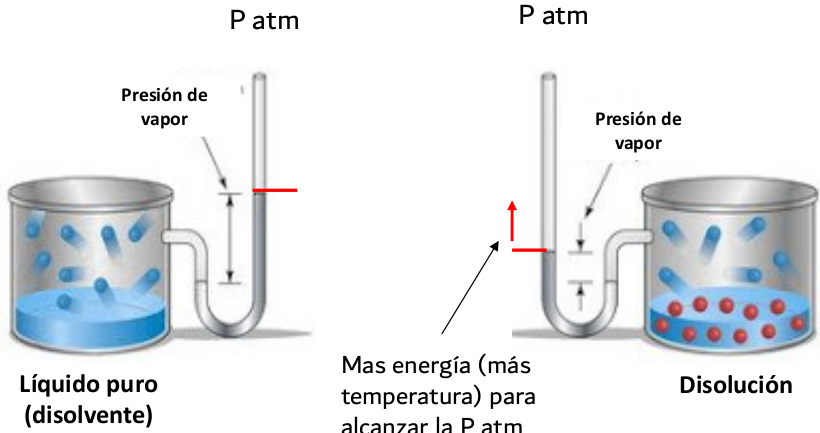
\includegraphics[scale=0.33]{foto/foto18.png}
\caption{Aumento del punto de ebullición}
\end{figure}

Si la presión de vapor de una disolución es menor respecto a la del disolvente puro, será necesaria un mayor cantidad de calor (mayor temperatura) para que esta presión alcance la presión atmosférica externa.

\begin{equation}
\Delta T_{b}=K_{b}m
\end{equation}

$\Delta T_{b}$ variación de la temperatura de ebullición. $K_{b}$ constante ebulloscópica (boiling constant). $m$ molalidad

\begin{equation}
\Delta T_{b}=T_{b}-T_{b}^{\circ}
\end{equation}



\subsection{Disminución del punto de congelación}
Temperatura a la cual coexisten en equilibrio las fases sólidad y líquida de una sustancia.

\begin{equation}
\Delta T_{f}=K_{f} \cdot m
\end{equation}

$\Delta T_{f}$ variación de la temperatura de congelación. $K_{f}$ constante crioscópica. $m$ molalidad

\begin{equation}
\Delta T_{f}=T_{f}-T_{f}^{\circ}
\end{equation}

\begin{figure}[H]
\center
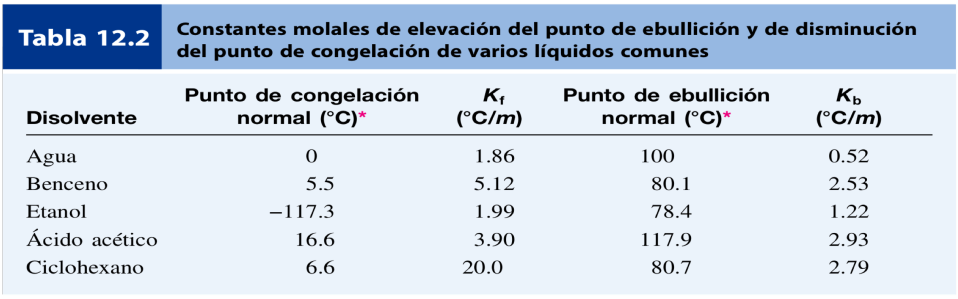
\includegraphics[scale=0.4]{foto/foto19.png}
\caption{tabla con las constantes ebulloscópica y crioscópica}
\end{figure}



\subsection{Presión osmótica}
Osmosis: Movimiento neto de las moléculas del disolvente desde una zona de menor concentración a una de mayor concentración a través de una membrana semipermeable.

\begin{figure}[H]
\center
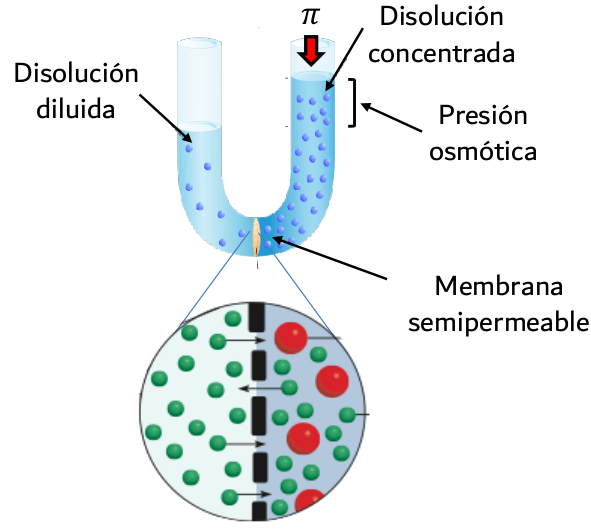
\includegraphics[scale=0.33]{foto/foto20.png}
\caption{Presión osmótica en una membrana}
\end{figure}

Presión osmótica ($\pi$): Presión que se requiere para detener la osmosis.

\begin{equation}
 \pi = M \cdot R \cdot T
 \end{equation} 

$M$ molaridad. $R=0.0821 \frac{atm \cdot L}{K \cdot mol}$. $T$ temperatura en kelvin.



\section{Propiedades coligativas en electrolitos}
Las propiedades coligativas dependen del \textbf{número de particulas} en la disolución. En las disoluciones de electrolitos esta propiedad dependerá de la \textbf{cantidad de iones} que cada soluto genere en la disolución.

\begin{figure}[H]
\center
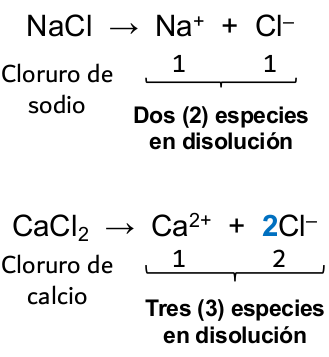
\includegraphics[scale=0.3]{foto/foto21.png}
\caption{ejemplo de disociación de electrolitos}
\end{figure}

Una medida del grado de disociacion en que los electrolitos se disocian es el \textbf{factor de van't hoff} $i$. El \textbf{valor ideal del factor de van't hoff} ($i$) para una sal se estima a partir del número de iones que se genera en la disolución por unidad formular.

\begin{equation}
i=\frac{\text{número real de partículas en disolución después de la disociación}}{\text{número de unidades de formulares inicialmnete disueltas en la disolución}}
\end{equation}

Sin embargo, las propiedades coligativas de las disoluciones de electrolitos son más pequeñas de lo que se esperaría, porque a concentraciones elevadas intervienen las fuerzas electroestáticas y se pueden formar pares iónicos.

\begin{figure}[H]
\center
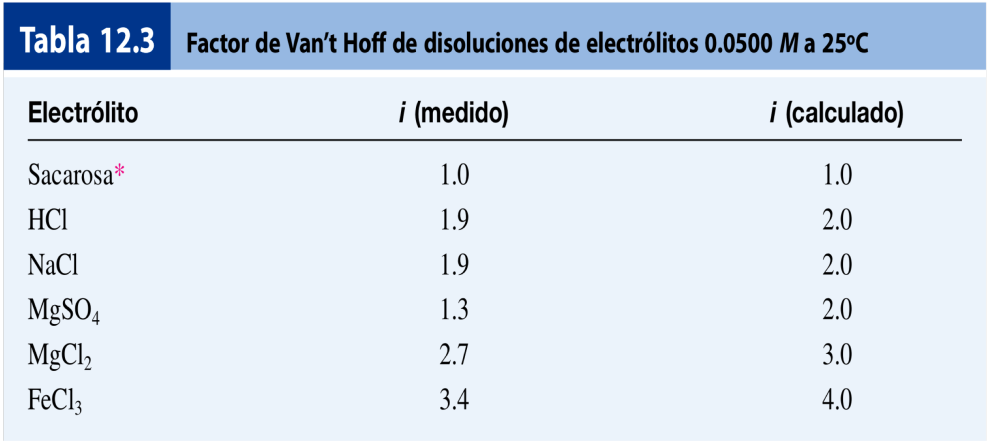
\includegraphics[scale=0.3]{foto/foto22.png}
\caption{factor de van't hoff experimental vs ideal}
\end{figure}

Al aplicar el factor de van't hoff a las ecuaciones de las propiedades coligativas obtenemos

\begin{equation}
\Delta T_{b}=iK_{b}m
\end{equation}

\begin{equation}
\Delta T_{f}=iK_{f}m
\end{equation}

\begin{equation}
\pi = iMRT
\end{equation}



\part{Clase 15}



\section{Tipos de equilibrio}
\begin{figure}[H]
\center
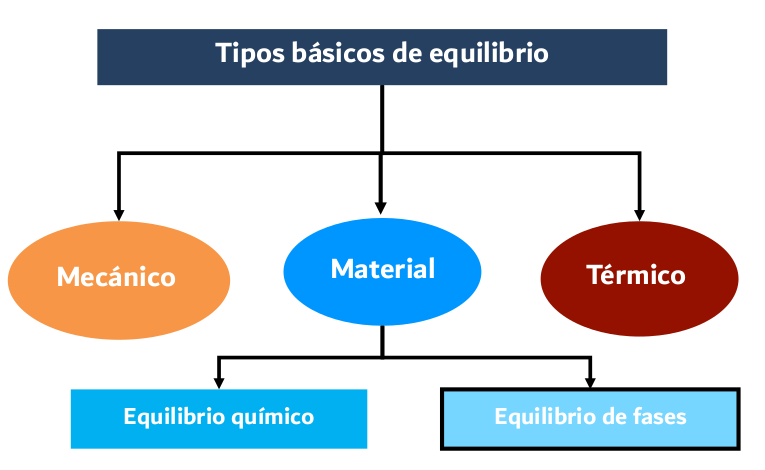
\includegraphics[scale=0.3]{foto/foto23.png}
\caption{Tipos de equilibrio}
\end{figure}

El \textbf{equilibrio material} se alcanza cuando un sistema se encuentra en equilibrio químico y en equilirbio de fases. No hay cambio global en la composición del sistema ni transferencia neta de materia.



\subsection{Equilibrio material}

Se alcanza cuando en cada fase de un sistema cerrado, el número de moles de cada sustancia resente no varía a lo largo del tiempo.

\begin{figure}[H]
\center
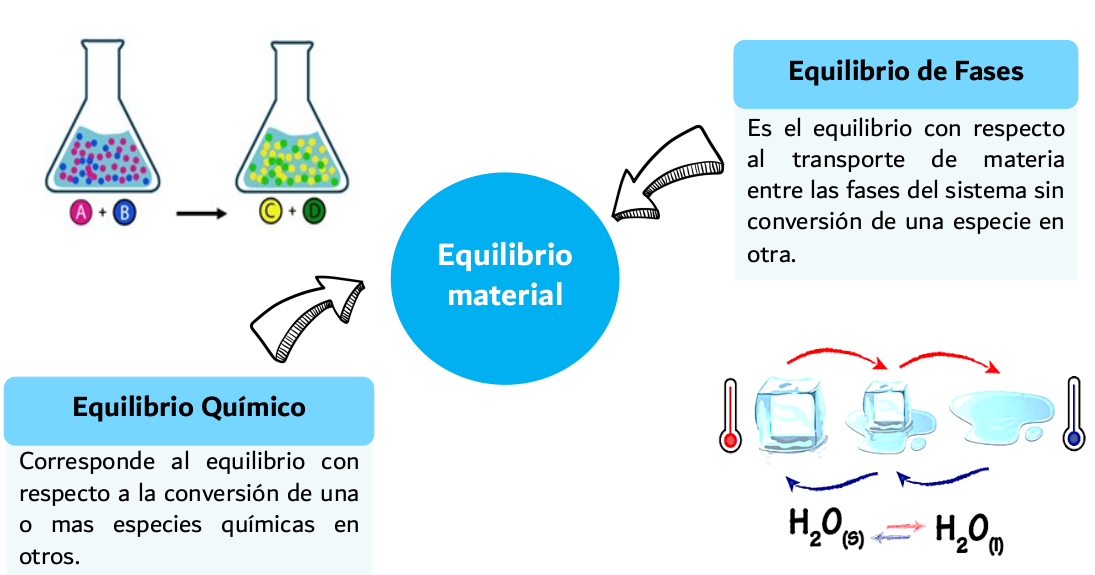
\includegraphics[scale=0.35]{foto/foto24.png}
\end{figure}



\section{Cambios de fases}
Los cambios de fase se presentan cuando se agrega o se quita energía (casi siempre en forma de calor).
\begin{figure}[H]
\center
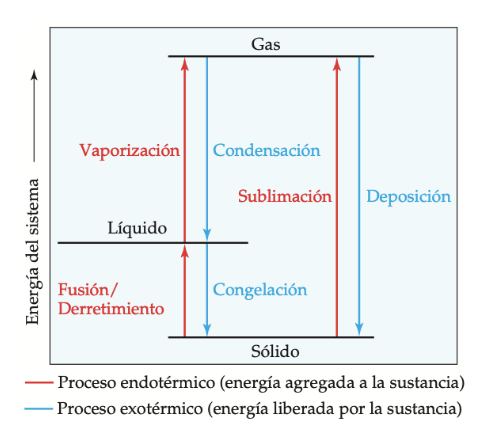
\includegraphics[scale=0.42]{foto/foto25.png}
\caption{Energía del sistema en cambios de fase}
\end{figure}

Los cambios de fase son cambios físicos que se distinguen porque cambia el orden molecular, en la fase sólida las moléculas alcanzan el máximo ordenamiento, y en la fase gaseosa tienen el mayor desorden.



\section{Equilibrio líquido-vapor}
\begin{itemize}
	\item Si se calienta un líquido, sus moléculas aumentan su energía cinética ($E_{c}$)
	\item Si la $E_{c}$ es lo suficientemente grande, las moléculas comenzarán a escapar de la fase líquida (desde la superficie del líquido), y pasarán a la fase de vapor.
\end{itemize}

\begin{figure}[H]
\center
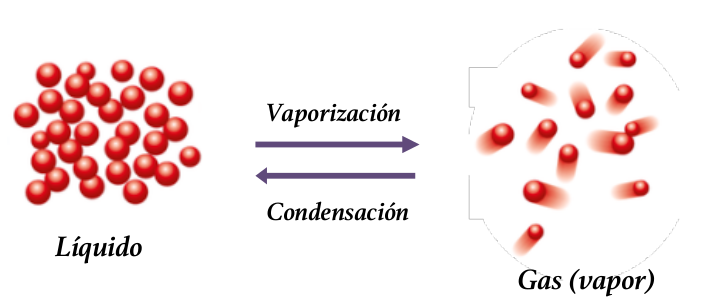
\includegraphics[scale=0.35]{foto/foto26.png}
\caption{cambio de fase líquido-vapor}
\end{figure}

Cuando las moléculas de un líquido tienen suficiente energía para escapar de la superficie, sucede un cambio de fase.




\end{document}




